\documentclass[12pt]{article}
\usepackage{amsmath}
\usepackage{amssymb}
\usepackage{amsthm}
\usepackage{amsfonts}
\usepackage{graphicx} 
\graphicspath{{./images/}}

\title{Homework 9 7.8II, 11.1I, 11.1II}
\author{Rafael Betita\\
MATH 005BH - Single Variable Calculus II}

\begin{document}
\maketitle

\newpage\section{Section 7.8 II }
p.575 (49, 50, 51, 55, 57)
\begin{enumerate}
    \addtocounter{enumi}{48}
    \item$\int_0^\infty\frac{x}{x^3+1}dx$
        \begin{align*}
            \frac{x}{x^3+1} \leq \frac{x}{x^3} && \frac{x}{x^3} = \frac{1}{x^2}
            && \int_1^\infty\frac{1}{x^2}dx \text{ converges}
        \end{align*}
        \begin{align*}
            \int_0^\infty\frac{x}{x^3+1}dx = \int_0^1\frac{x}{x^3+1}dx + \int_1^\infty\frac{x}{x^3+1}dx
        \end{align*}
        \begin{align*}
            \int_1^\infty\frac{1}{x^2}dx \text{ converges, therefore }  \int_0^\infty\frac{x}{x^3+1}dx \text{ also converges}
        \end{align*}
    \item $\int_1^\infty\frac{1+\sin^2x}{\sqrt{x}}dx$
        \begin{align*}
            0 \leq \sin^2x \leq 1 && \int_1^\infty \frac{1+0}{\sqrt{x}}dx \leq \int_1^\infty \frac{1+\sin^2x}{\sqrt{x}}dx
        \end{align*}
        \begin{align*}
             \int_1^\infty \frac{1}{x^{1/2}}dx \text{ is divergent, therefore, original equation is also divergent}
        \end{align*}
    \item $\int_1^\infty\frac{x+1}{\sqrt{x^4-x}}dx$
        \begin{align*}
            \frac{x+1}{\sqrt{x^4-x}} \geq 
            \frac{x}{\sqrt{x^4}} \geq
            \frac{1}{x^2}
        \end{align*}
        \begin{align*}
            \text{$\int_1^\infty\frac{1}{x^2}dx$ is divergent, therefore original equation is also divergent}
        \end{align*}
    \newpage\addtocounter{enumi}{3}\item $\int_0^\infty\frac{1}{\sqrt{x}(1+x)}dx$ \quad \\\\\intertext{The interval is improper for two reasons: The interval $[0, \infty)$ is infinite and the integrand has an infinite discontinuity at 0. Evaluate it by expressing it as a sum of improper integrals of Type 2 and Type 1 as follows:}\\
    \begin{align*}
        \int_0^\infty\frac{1}{\sqrt{x}(1+x)}dx = && 
        \int_0^1\frac{1}{\sqrt{x}(1+x)}dx + 
        \int_1^\infty\frac{1}{\sqrt{x}(1+x)}dx
    \end{align*}
    \begin{align*}
        \int_0^\infty\frac{1}{\sqrt{x}(1+x)}dx=\lim_{t\to 0^+}\int_t^1\frac{1}{\sqrt{x}(1+x)}dx+
        \lim_{t\to \infty}\int_1^\infty\frac{1}{\sqrt{x}(1+x)}dx
    \end{align*}
    \begin{align*}
        u &= \sqrt{x}
        \\ u^2 &= x
        \\2udu &= dx
    \end{align*}
    \begin{align*}
        \int\frac{2udu}{u(1+u^2)} = 2\int\frac{du}{1+u^2} = 2\arctan u + C = 2\arctan \sqrt{x} + C \\
        \lim_{t\to 0^+} 2\arctan\sqrt{x} \bigg|_t^1 + 
        \lim_{t\to \infty} 2\arctan\sqrt{x} \bigg|_1^t = \left[2\left(\frac{\pi}{4}-0\right) + 2\left(\frac{\pi}{2}-\frac{\pi}{4}\right)\right] = \pi
    \end{align*}
    \newpage\addtocounter{enumi}{1}\item $\int_0^1\frac{1}{x^p}dx$
    \begin{align*}
        p &= 1: \lim_{t\to\ 0^+}\int_0^1\frac{1}{x}dx = \lim_{t\to\ 0^+} \ln{x}\bigg|_t^1 = 0 + \infty \\
        p &= 0
    \end{align*}
\end{enumerate}

\newpage\section{Section 11.1 I}
p.744-745 (1, 2, 5-53 EOO, 73, 75)
\begin{enumerate}
    \item
        \begin{enumerate}
            \item What is a sequence?\\\\
                A sequence is a list of numbers that is written in a definite order. For every positive integer n, there is a corresponding number of $a_n$.\\
            \item What does it mean to say that $\lim_{n\to\infty}a_n = 8$?
                \\\\ As n approaches infinity, the series converges to a limit of 8.\\
            \item What does it mean to say that $\lim_{n\to\infty}a_n = \infty$?
                 As n approaches infinity, the series diverges to a limit of infinity.\\
        \end{enumerate}
    \item
        \begin{enumerate}
            \item What is a convergent sequence? Give two examples. 
                \\\\ A convergent sequence is a sequence for which a limit exists as n approaches infinity. An example would be $\frac{n+1}{2n^2}$ or $\frac{1}{n}$ \\
            \item What is a divergent sequence? Give two examples.
                \\\\ A convergent sequence is a sequence for which its limit does not exist as n approaches infinity. An example would be $27^n$ or $n$ \\
        \end{enumerate}
    \addtocounter{enumi}{2}\item $a_n=\frac{(-1)^{n-1}}{5^n}$
        \begin{equation*}
            \left[\frac{1}{5}, -\frac{1}{25}, \frac{1}{125}, -\frac{1}{625}, \frac{1}{3125}\right]
        \end{equation*}
    \addtocounter{enumi}{3}\item $a_1=1,\ a_{n+1}=5a_n-3$
        \begin{equation*}
            \left[1,2,7,32,157 \right]
        \end{equation*}
        
    \newpage Find a formula for the general term $a_n$ of the sequence assuming that the pattern of the first few terms continues..
    \addtocounter{enumi}{3}\item $\left\{\frac{1}{2},\frac{1}{4},\frac{1}{6}, \frac{1}{8}, \frac{1}{10}, ...\right\}$
        \begin{equation*}
            \frac{1}{2n}
        \end{equation*}
    \addtocounter{enumi}{3}\item 
    $\left\{\frac{1}{2},-\frac{4}{3},\frac{9}{4},-\frac{16}{5},\frac{25}{6},...\right\}$
        \begin{equation*}
            \frac{(-1)^{n-1} \cdot n^2}{1+n}
        \end{equation*}
    \addtocounter{enumi}{3}\item $a_n=1+(-\frac{1}{2})^n$
    \begin{align*}
        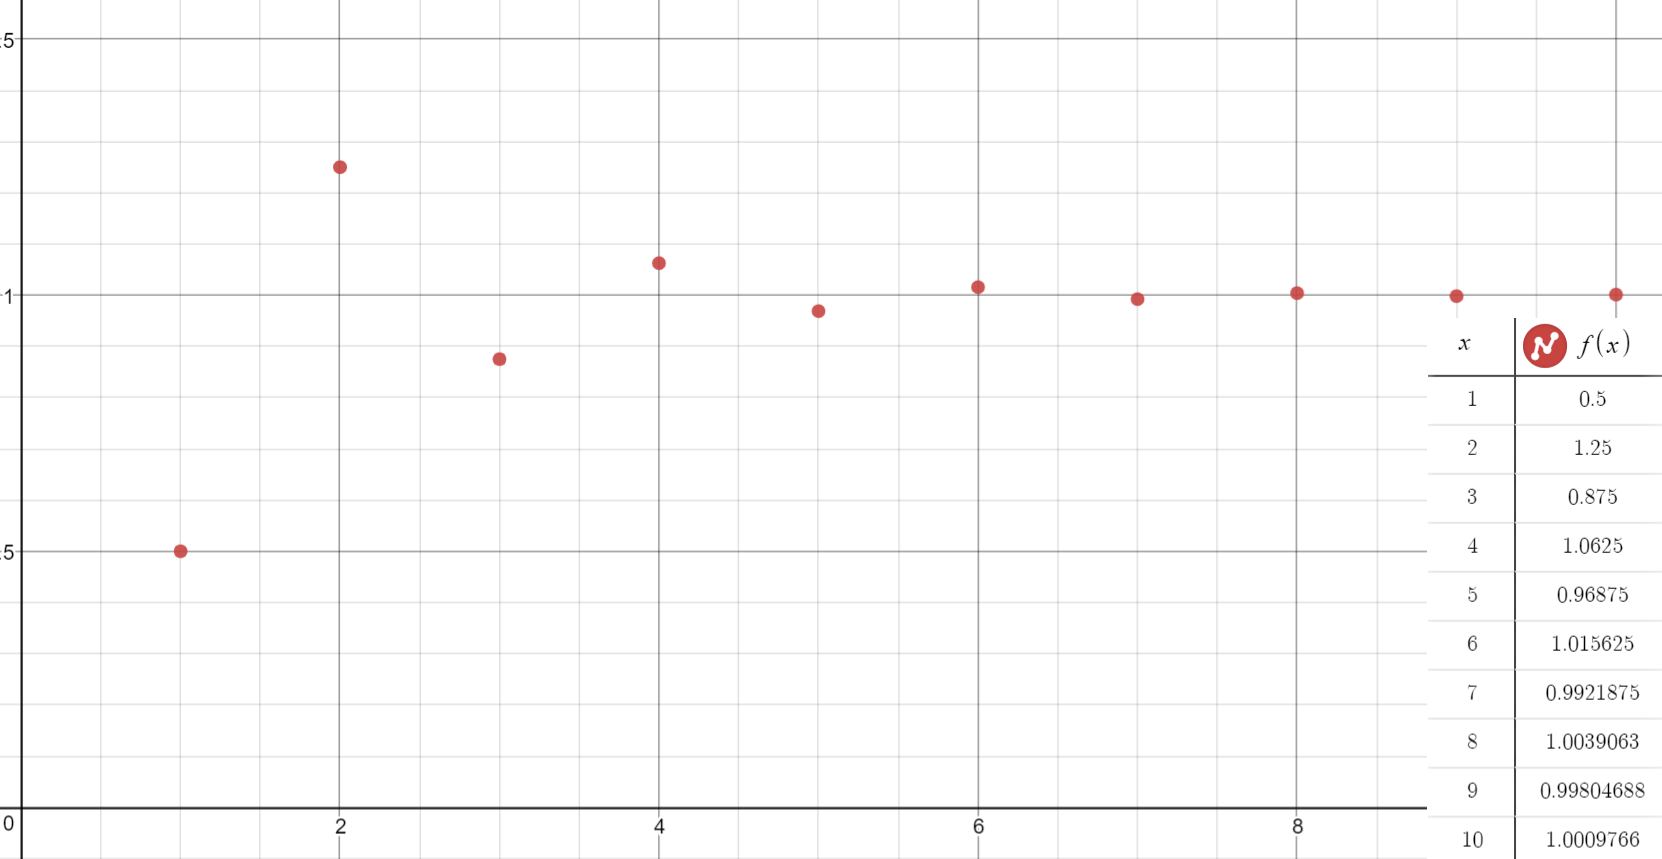
\includegraphics[width=\textwidth]{21}
    \end{align*}
        The sequence converges to 1.
    \begin{align*}
       \lim_{n\to\infty}\left(1+\left(-\frac{1}{2}^n\right)\right) = 1 + 0
    \end{align*}     
    \addtocounter{enumi}{3}\item $\frac{n^4}{n^3-2n}$
    \begin{align*}
        \left\{\right\}
    \end{align*}
    \addtocounter{enumi}{3}\item $a_n=e^{-1/\sqrt{n}}$
    \addtocounter{enumi}{3}\item $a_n=\frac{n^2}{\sqrt{n^3+4n}}$
    \addtocounter{enumi}{3}\item $\left\{\frac{(2n-1)!}{(2n+1)!}\right\}$
    \addtocounter{enumi}{3}\item $\{n^2e^{-n}\}$
    \addtocounter{enumi}{3}\item $a_n=n\sin(1/n)$
    \addtocounter{enumi}{3}\item $a_n=\ln{(2n^2+1)}-\ln{(n^2+1)}$
    \addtocounter{enumi}{3}\item $\left\{0,1,0,0,1,0,0,0,1,...\right\}$\\\\
    
    Determine whether the sequence is increasing, decreasing, or not monotonic. Is the sequence bounded?
    \addtocounter{enumi}{19}\item $a_n=\frac{1}{2n+3}$\\\\
    The sequence is decreasing as n approaches $\infty$. The sequence is also bounded between 0 and $\frac{1}{5}$.
    \addtocounter{enumi}{1}\item $a_n=n(-1)^n$\\\\
    The sequence is increasing as n approaches $\infty$. The sequence is also not bounded since it alternates between signs and and approaches $\infty$ on both bounds.
    
    
\end{enumerate}

\end{document}
